
\documentclass[12pt,a4paper]{article}
\usepackage[slovene]{babel}
\usepackage[utf8]{inputenc}
\usepackage[T1]{fontenc}
\usepackage{amsmath}
\usepackage{pgfplots}
\pgfplotsset{width=0.9\textwidth, compat=1.18}
\usepackage{pgf-pie}
\usepackage{booktabs}
\usepackage{caption}

\title{Statistična analiza metov kocke}
\author{}
\date{}

\begin{document}

\maketitle

\section{Naloga}

Generiran je bil naključni seznam 40 metov pravilne šeststrane kocke. Rezultati so naslednji:

\begin{center}
4, 6, 2, 5, 3, 1, 6, 4, 5, 2, \\
3, 6, 1, 4, 5, 3, 2, 6, 4, 1, \\
5, 3, 2, 6, 4, 1, 5, 3, 2, 6, \\
4, 1, 5, 3, 2, 6, 4, 1, 5, 3
\end{center}

\section{Frekvenčna porazdelitev}

\begin{table}[h]
\centering
\caption{Frekvenčna tabela metov kocke}
\begin{tabular}{cccc}
\toprule
Število pik & Frekvenca ($f_i$) & Relativna frekvenca ($f_i^0$) & Relativna frekvenca (\%)\\
\midrule
1 &  & \phantom{0.15} & \phantom{0.15} \\
2 &  &  & \phantom{0.15} \\
3 &  &  &  \\
4 &  &  & \\
5 &  &  & \\
6 &  &  &  \\
\midrule
Skupaj &  &  &   \\
\bottomrule
\end{tabular}
\end{table}

\section{Osnovni statistični kazalci}

\subsection{Srednja vrednost (aritmetična sredina)}


\bar{x} = \dfrac{\sum_{i=1}^{n}f_i x_i}{n} = 
$

\subsection{Mediana}
Urejen podatki:


Ker je $n=40$ sodo število, je mediana (Me):

$$\text{Me}=
$$

\subsection{Modus}
Modus je \rule{10cm}{0.1mm} 

\section{Grafični prikaz}

\begin{figure}[h]
\centering
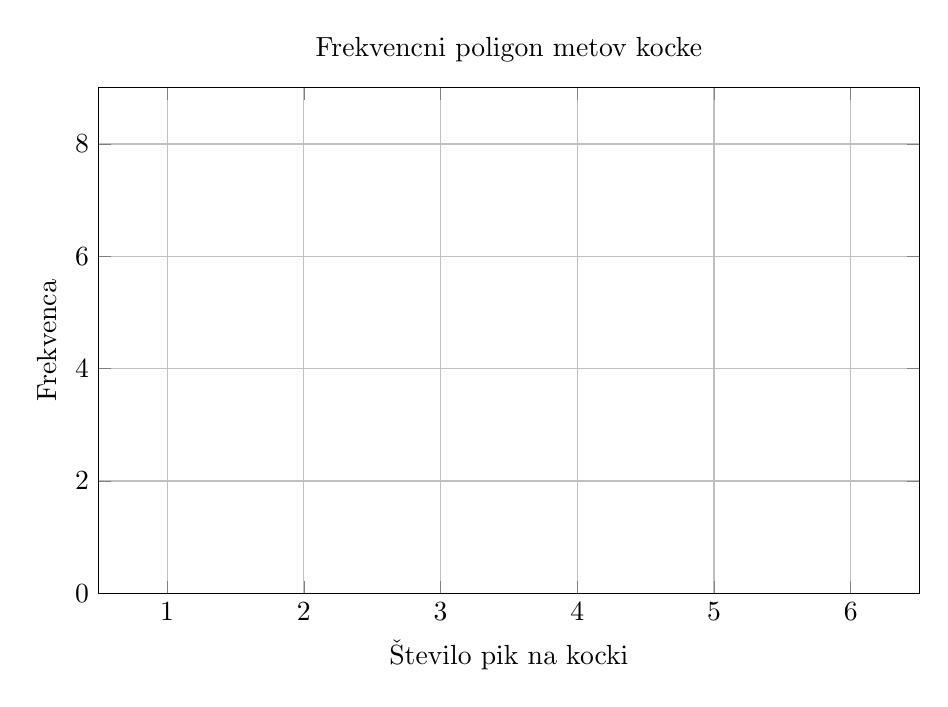
\begin{tikzpicture}
\begin{axis}[
    title={Frekvencni poligon metov kocke},
    xlabel={Število pik na kocki},
    ylabel={Frekvenca},
    xmin=0.5, xmax=6.5,
    ymin=0, ymax=9,
    xtick={1,2,3,4,5,6},
    grid=major,
    width=12cm,
    height=8cm,
    smooth,
    mark=*,
    mark size=2pt
]
\addplot[blue, thick] coordinates {
    %(1,6)
    %(2,7)
    %(3,8)
    %(4,7)
    %(5,7)
    %(6,5)
};
\end{axis}
\end{tikzpicture}
\caption{Frekvencni poligon prikazuje porazdelitev metov kocke}
\end{figure}

\newpage

\section{Naloga}

Zbrane so bile meritve oddaljenosti 100 naključno izbranih dijakov od šole (v kilometrih - km). Celoten seznam meritev je prikazan v tabeli.

Analizo oddaljenosti moramo razporediti v 5 statističnih razredov. Uporabite razrede s širino $h = 3$ km, začenši z vrednostjo 0,0 km (zaprti na levi, odprti na desni).

\normalsize % Prilagoditev velikosti pisave za obsežno tabelo podatkov
\begin{center}
\captionof{table}{Oddaljenost 100 dijakov od šole (v km)}
\begin{tabular}{|*{10}{c|}}
\hline
0,5 & 3,2 & 6,1 & 9,3 & 12,1 & 1,5 & 4,8 & 7,7 & 11,5 & 14,0 \\
\hline
1,2 & 4,5 & 7,5 & 11,2 & 13,9 & 2,8 & 5,9 & 8,4 & 10,9 & 13,3 \\
\hline
2,8 & 5,1 & 8,2 & 10,5 & 14,7 & 0,9 & 3,3 & 6,0 & 9,0 & 14,5 \\
\hline
0,9 & 3,8 & 6,7 & 9,8 & 12,5 & 1,5 & 4,1 & 7,3 & 11,1 & 12,9 \\
\hline
1,5 & 4,9 & 8,8 & 11,9 & 14,0 & 2,1 & 5,3 & 8,9 & 10,7 & 13,0 \\
\hline
2,1 & 5,5 & 7,1 & 10,1 & 13,3 & 0,4 & 3,9 & 6,2 & 9,5 & 14,1 \\
\hline
0,4 & 3,1 & 6,5 & 9,5 & 14,5 & 1,7 & 4,6 & 8,1 & 11,9 & 12,5 \\
\hline
1,7 & 4,2 & 8,1 & 11,5 & 12,9 & 2,9 & 5,7 & 6,9 & 9,8 & 14,7 \\
\hline
2,9 & 5,8 & 6,9 & 10,9 & 13,0 & 0,7 & 3,0 & 7,9 & 10,1 & 13,9 \\
\hline
0,7 & 3,7 & 7,9 & 9,0 & 14,1 & 1,8 & 4,4 & 8,5 & 9,3 & 12,1 \\
\hline
1,8 & 4,4 & 8,5 & 11,1 & 12,5 & 2,3 & 5,0 & 6,3 & 11,2 & 14,0 \\
\hline
2,3 & 5,0 & 6,3 & 10,7 & 14,0 & 0,6 & 3,5 & 7,3 & 10,5 & 13,3 \\
\hline
0,6 & 3,5 & 7,3 & 9,3 & 14,5 & 1,4 & 4,8 & 8,9 & 10,9 & 12,9 \\
\hline
1,4 & 4,8 & 8,9 & 11,2 & 12,9 & 2,5 & 5,9 & 6,0 & 9,0 & 13,0 \\
\hline
2,5 & 5,9 & 6,0 & 10,5 & 13,0 & 0,8 & 3,3 & 7,7 & 11,5 & 14,7 \\
\hline
0,8 & 3,3 & 7,7 & 9,8 & 14,7 & 1,3 & 4,1 & 8,4 & 10,7 & 12,5 \\
\hline
1,3 & 4,1 & 8,4 & 10,1 & 12,5 & 2,6 & 5,3 & 6,2 & 9,5 & 13,9 \\
\hline
2,6 & 5,3 & 6,2 & 9,5 & 13,9 & 0,3 & 3,9 & 6,7 & 11,9 & 14,0 \\
\hline
0,3 & 3,9 & 6,7 & 10,7 & 14,0 & 1,9 & 4,6 & 8,8 & 10,1 & 13,3 \\
\hline
1,9 & 4,6 & 8,8 & 11,9 & 13,3 & 2,2 & 5,7 & 7,1 & 9,8 & 14,5 \\
\hline
\end{tabular}
\end{center}
\normalsize

\section{Frekvenčna porazdelitev po razredih}

Izpolnite frekvenčno tabelo na podlagi zgornjih 100 podatkov. Celoten vzorec je $n=100$ dijakov.

\begin{table}[h]
\centering
\caption{Frekvenčna tabela oddaljenosti dijakov}
\begin{tabular}{ccccc}
\toprule
Razred (Oddaljenost)& Razredna sredina ($x'_i$) & Frekvenca ($f_i$) & Rel. frekvenca ($f_i^0$) \\
\midrule
$[0,0, 3,0)$ &  &  &  & \\
\midrule
$[3,0, 6,0)$ &  &  &  & \\
\midrule
$[6,0, 9,0)$ &  &  &  & \\
\midrule
$[9,0, 12,0)$ &  &  &  & \\
\midrule
$[12,0, 15,0)$&  &  &  & \\
\midrule
Skupaj   & \phantom{100} & & \\
\bottomrule
\end{tabular}
\end{table}

\section{Osnovni statistični kazalci}
Za izračun osnovnih statistik uporabite razredne sredine ($x'_i$).

\subsection{Srednja vrednost (aritmetična sredina)}

$$\bar{x} = \dfrac{\sum_{i=1}^{k}f_i x'_i}{n} = 
$$

\subsection{Mediana}
Najprej določite medianin razred.

Medianin razred je:
$$\text{Me interval} = 
$$

Nato izračunajte mediano s pomočjo formule:

$$ \text{Me} = L + \frac{\frac{n}{2} - F_{me-1}}{f_{me}} \cdot h = $$


\subsection{Modus}
Najprej določite modalni razred.

Modalni razred je:
$$\text{Mo interval} =
$$ 

Nato izračunajte modus s pomočjo formule:

$$ \text{Mo} = L + \frac{f_m - f_{m-1}}{(f_m - f_{m-1}) + (f_m - f_{m+1})} \cdot h = $$

\section{Grafični prikaz}

\begin{figure}[h]
\centering
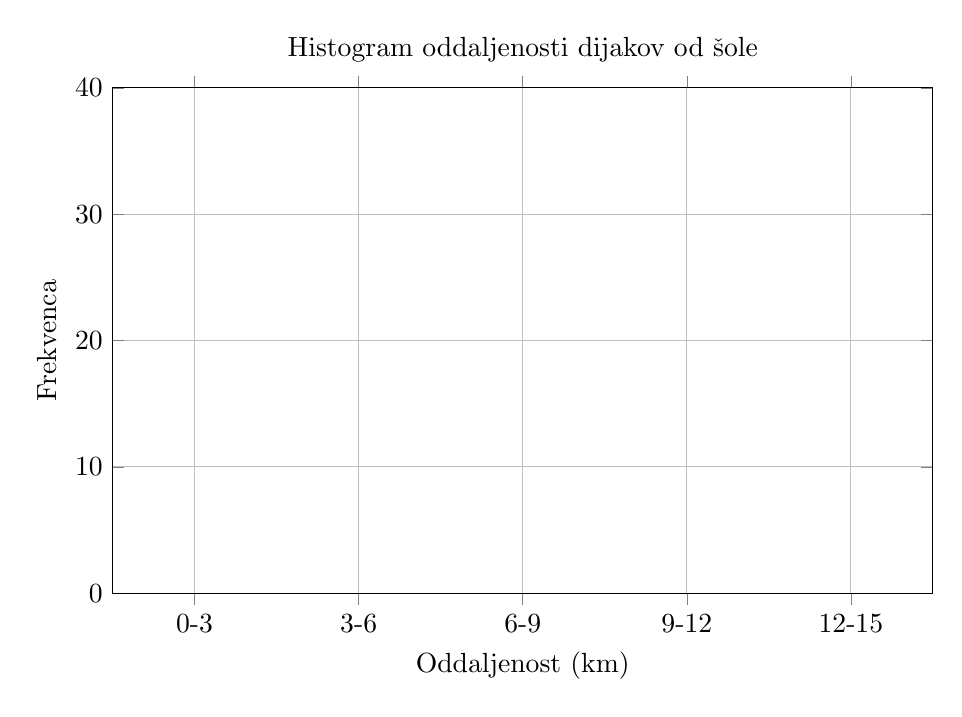
\begin{tikzpicture}
\begin{axis}[
    title={Histogram oddaljenosti dijakov od šole},
    xlabel={Oddaljenost (km)},
    ylabel={Frekvenca},
    xmin=0, xmax=15,
    ymin=0, ymax=40,
    xtick={1.5, 4.5, 7.5, 10.5, 13.5}, % Razredne sredine
    xticklabels={0-3, 3-6, 6-9, 9-12, 12-15}, 
    grid=major,
    width=12cm,
    height=8cm,
    ybar, % Uporaba histograma
    bar width=2.8cm, % Širina stolpca (malo manj kot širina razreda 3)
]
\addplot coordinates {
    %(1.5, f1)
    %(4.5, f2)
    %(7.5, f3)
    %(10.5, f4)
    %(13.5, f5)
};
\end{axis}
\end{tikzpicture}
\caption{Histogram prikazuje porazdelitev oddaljenosti dijakov (Podatki za stolpce se vnesete iz frekvenčne tabele)}
\end{figure}

\end{document}
\end{document}
\begin{figure}[h]
\centering
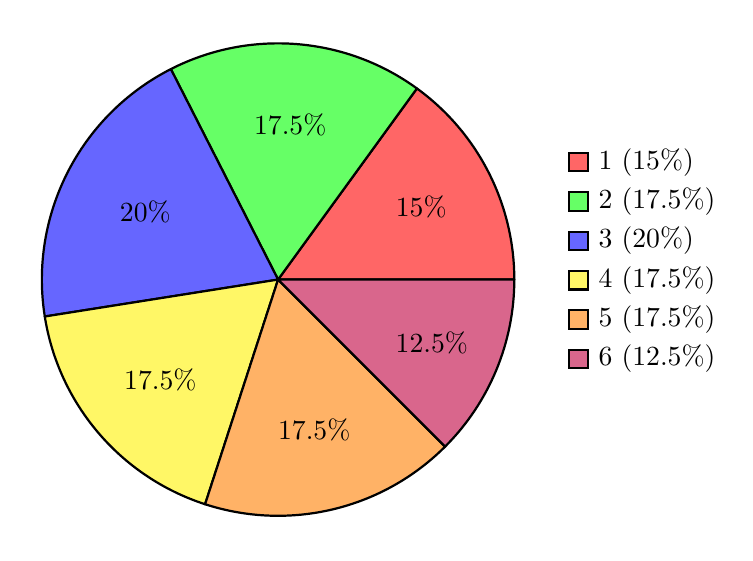
\begin{tikzpicture}
\pie[text=legend, radius=3, color={red!60, green!60, blue!60, yellow!60, orange!60, purple!60}]{
    15/1 (15\%),
    17.5/2 (17.5\%),
    20/3 (20\%),
    17.5/4 (17.5\%),
    17.5/5 (17.5\%),
    12.5/6 (12.5\%)
}
\end{tikzpicture}
\caption{Razsevni diagram relativnih frekvenc}
\end{figure}

\section{Zaključek}
Zapiši zaključke:
\vspace{5cm}


\end{document}


\documentclass[12pt,a4paper]{article}
\usepackage[slovene]{babel}
\usepackage[utf8]{inputenc}
\usepackage[T1]{fontenc}
\usepackage{amsmath}
\usepackage{pgfplots}
\pgfplotsset{width=0.9\textwidth, compat=1.18}
\usepackage{pgf-pie}
\usepackage{booktabs}
\usepackage{caption}

\title{Statistična analiza metov kocke}
\author{}
\date{}

\begin{document}

\maketitle

\section{Naloga}

Generiran je bil naključni seznam 40 metov pravilne šeststrane kocke. Rezultati so naslednji:

\begin{center}
4, 6, 2, 5, 3, 1, 6, 4, 5, 2, \\
3, 6, 1, 4, 5, 3, 2, 6, 4, 1, \\
5, 3, 2, 6, 4, 1, 5, 3, 2, 6, \\
4, 1, 5, 3, 2, 6, 4, 1, 5, 3
\end{center}

\section{Frekvenčna porazdelitev}

\begin{table}[h]
\centering
\caption{Frekvenčna tabela metov kocke}
\begin{tabular}{cccc}
\toprule
Število pik & Frekvenca ($f_i$) & Relativna frekvenca ($rf_i$) & Relativna frekvenca (\%)\\
\midrule
1 & 6 & 0.15 & 15\% \\
2 & 7 & 0.175 & 17.5\% \\
3 & 8 & 0.2 & 20\% \\
4 & 7 & 0.175 & 17.5\% \\
5 & 7 & 0.175 & 17.5\% \\
6 & 5 & 0.125 & 12.5\% \\
\midrule
Skupaj & 40 & 1.00 & 100\% \\
\bottomrule
\end{tabular}
\end{table}

\section{Osnovni statistični kazalci}

\subsection{Srednja vrednost (aritmetična sredina)}
\[
\bar{x} = \frac{\sum_{i=1}^{n} x_i}{n} = \frac{1\cdot6 + 2\cdot7 + 3\cdot8 + 4\cdot7 + 5\cdot7 + 6\cdot5}{40} = \frac{142}{40} = 3.55
\]

\subsection{Mediana}
Urejen podatek: 1,1,1,1,1,1, 2,2,2,2,2,2,2, 3,3,3,3,3,3,3,3, 4,4,4,4,4,4,4, 5,5,5,5,5,5,5, 6,6,6,6,6

Ker je $n=40$ sodo število, je mediana povprečje 20. in 21. vrednosti:
\[
\text{Mediana} = \frac{3 + 4}{2} = 3.5
\]

\subsection{Modus}
Modus je vrednost z največjo frekvenco: $\text{Modus} = 3$ (frekvenca 8)

\section{Grafični prikaz}

\begin{figure}[h]
\centering
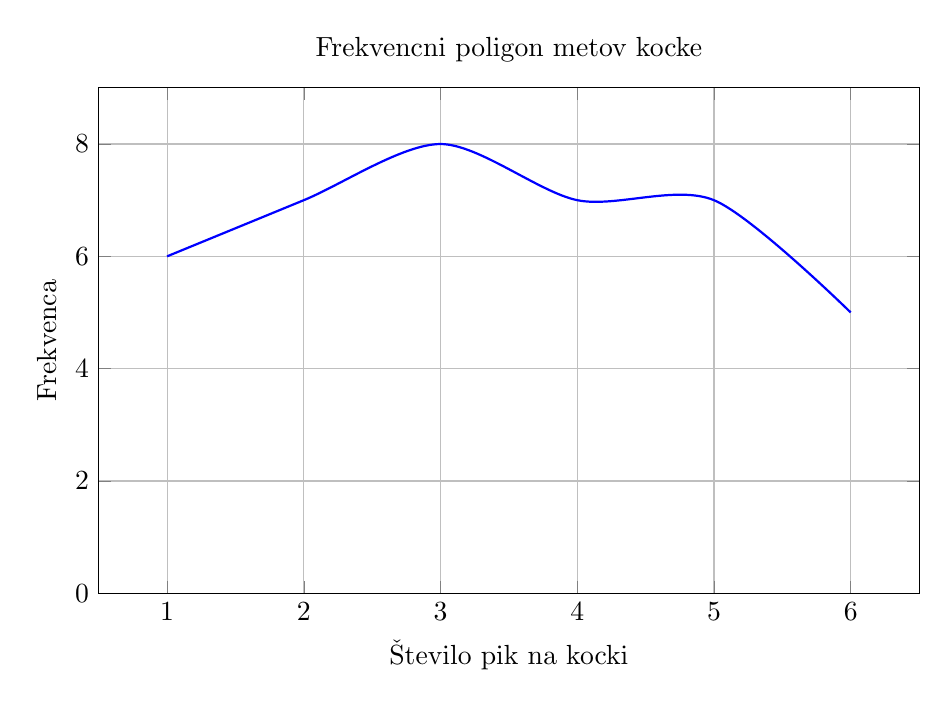
\begin{tikzpicture}
\begin{axis}[
    title={Frekvencni poligon metov kocke},
    xlabel={Število pik na kocki},
    ylabel={Frekvenca},
    xmin=0.5, xmax=6.5,
    ymin=0, ymax=9,
    xtick={1,2,3,4,5,6},
    grid=major,
    width=12cm,
    height=8cm,
    smooth,
    mark=*,
    mark size=2pt
]
\addplot[blue, thick] coordinates {
    (1,6)
    (2,7)
    (3,8)
    (4,7)
    (5,7)
    (6,5)
};
\end{axis}
\end{tikzpicture}
\caption{Frekvencni poligon prikazuje porazdelitev metov kocke}
\end{figure}

\begin{figure}[h]
\centering
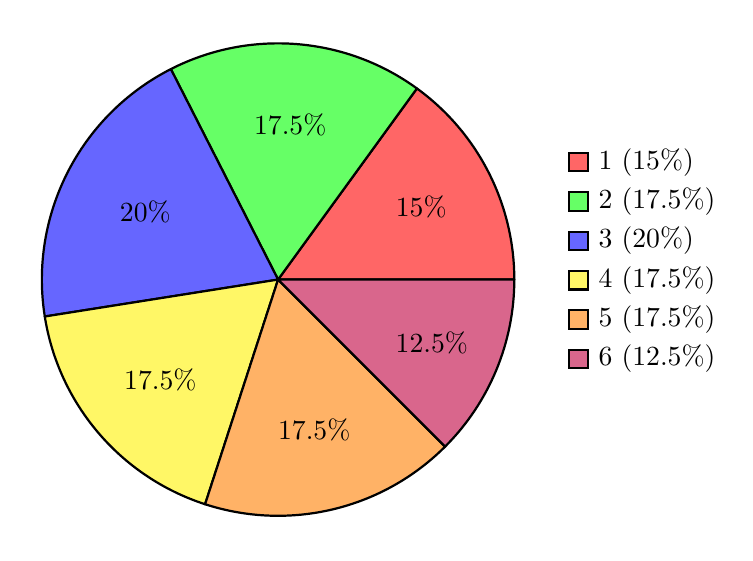
\begin{tikzpicture}
\pie[text=legend, radius=3, color={red!60, green!60, blue!60, yellow!60, orange!60, purple!60}]{
    15/1 (15\%),
    17.5/2 (17.5\%),
    20/3 (20\%),
    17.5/4 (17.5\%),
    17.5/5 (17.5\%),
    12.5/6 (12.5\%)
}
\end{tikzpicture}
\caption{Razsevni diagram relativnih frekvenc}
\end{figure}

\section{Zaključek}
Analiza 40 metov kocke je pokazala, da so se številke pojavile relativno enakomerno, z majhno prednostjo številke 3. Srednja vrednost 3.55 in mediana 3.5 kažeta na simetrično porazdelitev. Modus 3 se je pojavil 8-krat, kar je 20\% vseh metov.

\end{document}